% Choose one to switch between slides and handout
\documentclass[]{beamer}
%\documentclass[handout]{beamer}

% Video Meta Data
\title{Bitcoin, Blockchain and Cryptoassets}
\subtitle{Introduction to Consensus}
\author{Prof. Dr. Fabian Schär}
\institute{University of Basel}

% Config File
% Packages
\usepackage[utf8]{inputenc}
\usepackage{hyperref}
\usepackage{gitinfo2}
\usepackage{tikz}
\usepackage{amsmath}
\usepackage{bibentry}
\usepackage{xcolor}
\usepackage{colortbl} % Add colour to LaTeX tables
\usepackage{caption}
\usepackage[export]{adjustbox}
\usepackage{pgfplots} \pgfplotsset{compat = 1.17}

% Color Options
\definecolor{highlight}{rgb}{0.65,0.84,0.82}
\definecolor{focus}{rgb}{0.72, 0, 0}

% Beamer Template Options
\beamertemplatenavigationsymbolsempty
\setbeamertemplate{footline}[frame number]
\setbeamercolor{structure}{fg=black}
\setbeamercolor{footline}{fg=black}
\setbeamercolor{title}{fg=black}
\setbeamercolor{frametitle}{fg=black}
\setbeamercolor{item}{fg=black}
\setbeamercolor{}{fg=black}
\setbeamercolor{bibliography item}{fg=black}
\setbeamercolor*{bibliography entry title}{fg=black}
\setbeamertemplate{items}[square]
\setbeamertemplate{enumerate items}[default]
\captionsetup[figure]{labelfont={color=black},font={color=black}}
\captionsetup[table]{labelfont={color=black},font={color=black}}

\setbeamertemplate{bibliography item}{\insertbiblabel}

% Link Icon Command
\newcommand{\link}{%
    \tikz[x=1.2ex, y=1.2ex, baseline=-0.05ex]{%
        \begin{scope}[x=1ex, y=1ex]
            \clip (-0.1,-0.1)
                --++ (-0, 1.2)
                --++ (0.6, 0)
                --++ (0, -0.6)
                --++ (0.6, 0)
                --++ (0, -1);
            \path[draw,
                line width = 0.5,
                rounded corners=0.5]
                (0,0) rectangle (1,1);
        \end{scope}
        \path[draw, line width = 0.5] (0.5, 0.5)
            -- (1, 1);
        \path[draw, line width = 0.5] (0.6, 1)
            -- (1, 1) -- (1, 0.6);
        }
    }

% Read Git Data from Github Actions Workflow
% Defaults to gitinfo2 for local builds
\IfFileExists{gitInfo.txt}
	{\input{gitInfo.txt}}
	{
		\newcommand{\gitRelease}{(Local Release)}
		\newcommand{\gitSHA}{\gitHash}
		\newcommand{\gitDate}{\gitAuthorIsoDate}
	}

% Custom Titlepage
\defbeamertemplate*{title page}{customized}[1][]
{
  \vspace{-0cm}\hfill
\includegraphics[width=2.5cm]{../config/logo_cif}
  
\includegraphics[width=1.9cm]{../config/seal_wwz}
  \\ \vspace{2em}
  \usebeamerfont{title}\textbf{\inserttitle}\par
  \usebeamerfont{title}\usebeamercolor[fg]{title}\insertsubtitle\par  \vspace{1.5em}
  \small\usebeamerfont{author}\insertauthor\par
  \usebeamerfont{author}\insertinstitute\par \vspace{2em}
  \usebeamercolor[fg]{titlegraphic}\inserttitlegraphic
    \tiny \noindent \texttt{Release Ver.: \gitRelease}\\ 
    \texttt{Version Hash: \gitSHA}\\
    \texttt{Version Date: \gitDate}\\ \vspace{1em}
  \link \href{https://github.com/cifunibas/Bitcoin-Blockchain-Cryptoassets/blob/main/slides/intro.pdf}
  {Get most recent version}\\
  \link \href{https://github.com/cifunibas/Bitcoin-Blockchain-Cryptoassets/blob/main/slides/intro.pdf}
  {Watch video lecture}\\ \vspace{1em}
  License: \texttt{Creative Commons Attribution-NonCommercial-ShareAlike 4.0 International}\\\vspace{2em}
  
\includegraphics[width = 1.2cm]{../config/license}
}

% tikzlibraries
\usetikzlibrary{decorations.pathreplacing}
\usetikzlibrary{decorations.markings}
\usetikzlibrary{positioning}

%caption font
\captionsetup{font=footnotesize}


%%%%%%%%%%%%%%%%%%%%%%%%%%%%%%%%%%%%%%%%%%%%%%
%%%%%%%%%%%%%%%%%%%%%%%%%%%%%%%%%%%%%%%%%%%%%%
\begin{document}

\thispagestyle{empty}
\begin{frame}[noframenumbering]
	\titlepage
\end{frame}

%%%
\begin{frame}{Why Consensus Matters}

Distributed ledger as \color{focus} chain of transactions and states \color{black} whose \color{focus} compliance with an explicit rule set \color{black} is  attested by a reliable network of record keeping nodes.

\uncover<2->{
\vspace{1.5 em}
\textbf{Account statement example:}

\begin{center}
\begin{tikzpicture}[scale=0.7, every node/.style ={scale=0.8}]
		
% Agent Savvy
	\node 			(savvy) at (12,0) {
\includegraphics[height = 2cm]{../assets/images/agents/handing_left.png}};
	\node			(as_official) at (10,0) {
\includegraphics[height = 1.6 cm]{../assets/images/account_statement_official.png}};

% Agent Naive
	\node 			(naive) at (0,0) {
\includegraphics[height = 2 cm]{../assets/images/agents/handing_right.png}};
	\node			(as_DIY) at (2,0) {
\includegraphics[height = 1.8cm]{../assets/images/account_statement_handmade.png}};

% Text
	
	\node  			at (6,0) {\LARGE vs.};

		

\end{tikzpicture}
\end{center}

\vspace{1 em}

$\Rightarrow$ Value of the ledger content relies on the network attesting it.
}

\end{frame}
%%%	

%%%
\begin{frame}{Challenges for Reaching Consensus}

Two main challenges for consensus in a decentralized network:
	
	\begin{itemize}
		\item<1-> Each participant can adapt the ledger at its own discretion.
		\item<2-> No central authority to decide among two legitimate versions.
	\end{itemize}

\vspace{1 em}
\begin{center}
\begin{tikzpicture}[scale=0.8, every node/.style ={scale=0.8}]
		    
% Title: The two core challenges in finding Consensus


% Arrangement
	\coordinate (o0) at (0,2);
	\coordinate (o1) at (1,2);
	\coordinate (o2) at (3,2);
	\coordinate (o3) at (5,2);
	\coordinate (o4) at (7,2);

	\coordinate	(dm) at (5.9,4);

	\coordinate	(hm0) at (4,0);
	\coordinate (hm1) at (10,0);




% Chain
  \draw 		 (o0) -- (o1) -- (o2) -- (o3);
  \draw [dashed] (o3) -- (o4) ;
  \node (block1) at (o1) [fill=white,draw,minimum width=0.4cm,minimum height=0.4cm] {};
  \node (block2) at (o2) [fill=white,draw,minimum width=0.4cm,minimum height=0.4cm] {};
  \node (block3) at (o3) [fill=white,draw,minimum width=0.4cm,minimum height=0.4cm] {};
  \node (block4) at (o4) [fill=white,draw,dashed,minimum width=0.4cm,minimum height=0.4cm, text = focus] {\scriptsize ?};
  

% Dishonest Miner
	\node	(badminer) at (dm) {
\includegraphics[width = 1.2 cm]{../assets/images/agents/miner_devil.png}};
	\node	(invalidblock) at (badminer.east) {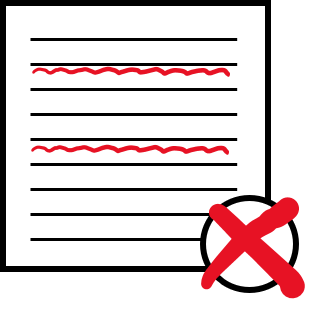
\includegraphics[width = 1 cm]{../assets/images/invalid_block.png}};
	\draw [->, thick, dashed, focus]	(invalidblock.south) -- (block4.north);

\uncover<2->{

% Honest Miners
 	\node	(goodminer0) at (hm0) {
\includegraphics[width = 1.2 cm]{../assets/images/agents/miner_right.png}};
 	\node 	(validblock0) at (goodminer0.east) {
\includegraphics[width = 1 cm]{../assets/images/valid_block.png}};
 	\draw [->,dashed,thick,focus]	(validblock0.north east) -- (block4.south west);
 	
 	\node	(goodminer1) at (hm1) {
\includegraphics[width = 1.2 cm]{../assets/images/agents/miner_left.png}};
 	\node 	(validblock1) at (goodminer1.west) {
\includegraphics[width = 1 cm]{../assets/images/valid_block.png}};
 	\draw [->,dashed,thick,focus]	(validblock1.north west) -- (block4.south east);

}	

\end{tikzpicture}
\end{center}

\end{frame}
%%%	

%%%
\begin{frame}{Measures Supporting Consensus}

\textbf{Explicit and unambiguous rule set} for legitimate changes to the ledger and block sequence.
\vspace{0.25 em}

$\Rightarrow$ Invalid blocks are detected easily and unambiguously.
\vspace{1.5 em}

\textbf{Decision mechanism} for consensus over different, legitimate extensions of the ledger. 
\vspace{0.25 em}

$\Rightarrow$ Swiftly resolving situations of uncertainty.
\vspace{1.5 em}

\textbf{Incentive system} that rewards compliant behaviour and / or penalizes manipulation attempts.
\vspace{0.25 em}

$\Rightarrow$ Typically in native protocol asset, tying the participant's interest to the sustainable value of the network.

	
\end{frame}
%%%

%%%
\begin{frame}{What Makes a Good Consensus Mechanism?}

Suitability of a consensus mechanism \color{focus} depends on the purpose and user base \color {black} of a decentralized ledger.
\vspace{1 em}

\textbf{The Trilemma:}

\begin{center}
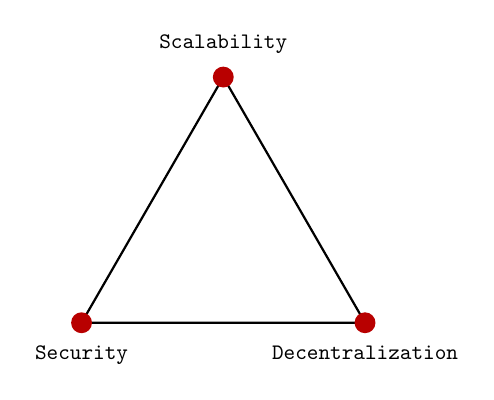
\begin{tikzpicture}[scale=0.6, every node/.style ={scale=0.8}]
		
% Title: Blockchain or Scalability Trilemma

% Arrangement
	\coordinate (A) at (0,0);
	\coordinate (B) at (3,5.2);
	\coordinate (C) at (6,0);


% Triangle
  \draw [thick]		 (A) -- (B) -- (C) -- (A);
  \node 			 at (A) [circle, fill = focus, minimum width=0.2cm,minimum height=0.2cm]{};
  	\node			 at	(A) [below = 0.2] {\texttt{Security}};
  \node 			 at (B) [circle, fill = focus, minimum width=0.2cm,minimum height=0.2cm]{};
  	\node			 at	(B) [above = 0.2] {\texttt{Scalability}};
  \node 			 at (C) [circle, fill = focus, minimum width=0.2cm,minimum height=0.2cm]{};
  	\node			 at	(C) [below = 0.2] {\texttt{Decentralization}};



\end{tikzpicture}
\end{center}

\textbf{Generalized Rule:} Subject to tadeoffs, i.e., not possible to achieve all three goals. 	
\end{frame}
%%%	


\end{document}